\documentclass[en]{../../../../../../eplexam}

\usepackage{pgfplots}
\pgfplotsset{compat=1.15}
\pdfminorversion=7

\hypertitle{Secure electronic circuits and systems}{8}{ELEC}{2760}{2019}{Juin}{All}
{Thomas Antoine \and Martin Braquet \and Romain Pattyn}
{François-Xavier Standaert}

During the written exam, it is possible to present/explain/detail on demand one (or both) question(s) to the professor.

\section{}
We consider the following Sbox:
$$S_{box}(a(x))=x\cdot\left(a(x)^{-1}\right) \mod p(x)$$
where $p(x) = x^4\oplus x\oplus 1$ to bring the output back in GF$(2^4)$.
\begin{enumerate}
    \item Implement the inverse as a function of products and squares only. Try to minimise the amount of such function calls because we will later use masking. Remember that $x^{-1} = x^{p^m-2}$ in GF$(p^m)$
    \item Why do we say that the square operator is $\oplus$-linear in a function characteristic 2. (hint: start by checking at $(x^2\oplus 1)^2 \mod p(x)$ and generalise it to any sum of polynomials.)
    \item Why can we say the same thing about the multiplication by the constant polynomial $c(x) = x$? (recall that this is equivalent to the XTime table of the exercise session)
    \item Build the table squaring table.
    \item By using an FPGA with logic blocks similar as the LB1 of the course (2 LUT of 4 bit, one multiplexer and 2 registers) what is the cost of the implementation in LB1 of the squaring table and the multiplication table? You can consider that you have access to those tables, for the square operator you have an $n$-bit by $n$-bit table and for the multiplication operator you have an $n_1$-bit by $n_2$-bit table.
    \item We want to mask the data with 3 shares, how many calls to the previous table implementations would you have to do for the square and multiplication operator?
\end{enumerate}

\begin{solution}
    \begin{enumerate}
        \item   We need to compute $x^{-1} = x^{2^4-2}=x^{14}$.
                We can begin by a series of squaring.
                \begin{align}
                    x^2 &= x\cdot x\\
                    x^4 &= x^2\cdot x^2\\
                    x^8 &= x^4\cdot x^4\\
                \end{align}
                We can then finish with the multiplications.
                \begin{align}
                    x^{12} &= x^8\cdot x^4\\
                    x^{14} &= x^{12}\cdot x^2\\
                \end{align}
        \item   Using the distributivity of the multiplication over the xor, we can see that
                $$(x^2\oplus 1)^2=(x^2\oplus 1)\cdot (x^2\oplus 1)=x^4 \oplus x^2 \cdot 1 \oplus 1 \cdot x^2 \oplus 1 =x^4 \oplus 1 $$
                Similarly for any polynomials $a(x)$ and $b(x)$ in GF$(2^4)$,
                $$(a(x)\oplus b(x))^2 = a(x)^2 \oplus a(x)\cdot b(x) \oplus b(x)\oplus a(x) \oplus b(x)^2 = a(x)^2 \oplus b(x)^2 $$
        \item   Once again, because of the distributivity property of the multiplication over the xor. For $a(x)$, $b(x)$, $c(x)\in GF(2^4)$, $$a(x)(b(x)\oplus c(x)) = a(x)b(x)\oplus a(x)c(x)$$. In our case, we can set $a(x)=x$ to get the desired result. In term of effect on the 4 bit number we saw during the practical session, it was equivalent to multiplying by two and then xoring with 19 ($x^4+x+1$) if it is bigger than 15. Both of those operations are $\oplus$-linear.
        \item   The table is as follows:
                \begin{center}
                    \begin{tabular}{c|c}
                        $x$ & $x^2$\\
                        \hline
                        0 & 0\\
                        1 & 1\\
                        2 & 4\\
                        3 & $1^2\oplus 2^2 = 1\oplus 4=5$\\
                        4 & 3\\
                        5 & $1^2 \oplus 4^2 = 1 \oplus 3=2$\\
                        6 & $2^2 \oplus 4^2 = 4\oplus 3=7$\\
                        7 & $3^2\oplus 4^2= 5\oplus 3=6$\\
                        8 & 12\\
                        9 & $1^2\oplus 8^2 = 1\oplus 12=13$\\
                        10 & $2^2\oplus 8^2 = 4 \oplus 12 = 8$\\
                        11 & $3^2 \oplus 8^2 = 5 \oplus 12 = 9$\\
                        12 & $4^2 \oplus 8^2 = 3 \oplus 12 = 15$\\
                        13 & $5^2 \oplus 8^2 = 2 \oplus 12 = 14$\\
                        14 & $6^2 \oplus 8^2 = 7 \oplus 12 = 11$\\
                        15 & $7^2 \oplus 8^2 = 6 \oplus 12 = 10$\\
                    \end{tabular}
                \end{center}
                If the input number is $a_3x^3\oplus a_2x^2\oplus a_1x\oplus a_0$. Then it can also be computed by
                \begin{equation}\label{formula_square}
                    (a_3x^6\oplus a_2x^4\oplus a_1x^2\oplus a_0)\oplus a_3 p(x)x^2 \oplus a_2 p(x) = a_3x^3\oplus (a_3\oplus a_1)x^2\oplus a_2x \oplus(a_0\oplus a_2)
                \end{equation}
                As a sanity check, we can observe that the square is a permutation and is thus invertible, as expected of a linear function.
        \item The look-up table for a square should have 4 bit as input while the multiplication should have 8. A 4 bit memory can be made via a single LB1 by branching the input bits to the input of the LUT and directly outputing the bit of the LUT. The 8 bit LUT of the multiplication can be made by 11 LB1 as seen in the course (and can be found in the "Synthèses" part of this drive).
        \item For a single share, using the algorithm given at the first part of this question, we would do  3 squaring and 2 multiplications. For 3 shares, we would do 9 squaring and 6 multiplications. This simple multiplication by the number of share simply comes from the linearity of our operations. This lets us reconstruct the result by xoring the result of the operations on each share.
    \end{enumerate}
\end{solution}

\section{}

Consider an encryption scheme where the Sbox is composed of a nonlinear function followed by a squaring operator. The output of the Sbox is then classically xored with the key. All the variables are expressed as 4-bit data (in GF($2^4$)).

\begin{figure}[H]
    \centering
    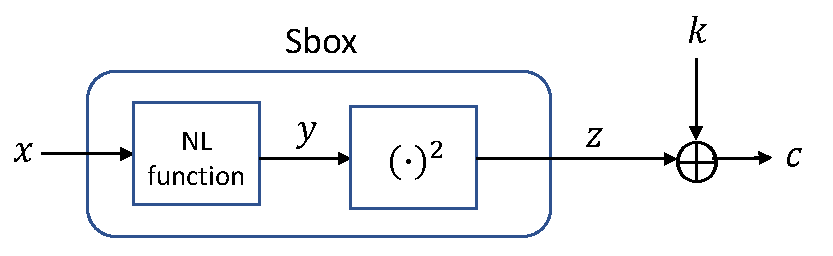
\includegraphics[width=0.6\textwidth]{Q2.pdf}
\end{figure}

\begin{enumerate}
    \item Is it possible to retrieve the key by inserting a toggling bit fault on $y$? If yes, how? If no, why?
    \item How many faults do we need to find the key by inserting a toggling bit fault on $x$ (i.e. a random bit of $x$ is toggled? The full encryption of a 128-bit key is composed of 32 encryption schemes in parallel, how many faults are required to find the full key? Explain.
    \item Now consider that the fault model is not so precise, so the fault toggles 2 random bits of $x$. How many faults are then needed to recover $k$? Explain your answer with theoretical information arguments. Hint: $C(4,2)=\binom{4}{2} = 6$ and $\log_2(6) \simeq 2.5$.
    \item \label{QL}
    We have at our disposal the (non-noisy) leakage $L$ of the 2 first bits of $z$: $L(z)="z_1z_0"$ ($z_i$ represents the $i$-th bit of $z$). How many encryptions do we need to recover the key?
    \item We have now at our disposal the (non-noisy) leakage $L$ of the 2 first bits of $x$: $L(x)="x_1x_0"$. The output\footnote{These numbers are given as an example, they were different in the exam.} of the Sbox is $$ [4,7,15,1,2,0,12,6,9,8,11,14,3,5,10,13].$$ Compute the key knowing that $c=0$ when $L="00"$, $c=1$ when $L="01"$ and $c=2$ when $L="11"$. 
    \item Which one of these (in)equalities is correct? Explain.
    \begin{align*}
        MI(x;L) & \le MI(k;L,c) \\
        MI(x;L) & =   MI(k;L,c) \\
        MI(x;L) & \ge MI(k;L,c)
    \end{align*}
    \item Compute $MI(x;L)$. Considering that $c=4$ in the formula given in the slides, compute the number of samples required to find the key. Is it in accordance to your answer of question \ref{QL}?
\end{enumerate}

\begin{solution}
    \begin{enumerate}
        \item   Taking the formula (\ref{formula_square}), we can see that toggling a bit of y is equivalent to toggling 1 or 2 bit of z.\smallskip

                However, this does not allow to find out the key as toggling bits of z will simply toggle the same bits of c, without giving us any information on k.
        \item   Let $c_f$ be the case with the fault, and $c$ the case without the fault. We can invert all of the operations on both of them to get $x_f$ and $x$.\smallskip

                Over the $2^4=16$ possible keys, there are only 4 where $HW(x,x_f) = 1$. (All operations are permutations).\smallskip

                We thus have $$MI(k, fault)= 4-2 = 2$$. We need approximately 2 faults to find the key.\smallskip

                Over the 128 bits, we have 32 times more keys, so we need 32 times more faults, so we need approximately 64 faults to find the full key.
        \item   We now have $C(4,2)=6$ possible combinations of 2 bits to toggle. We thus have $$MI(k, fault)= 4-\log_2{6} = 1.5$$ and we win 1.5 bit of information per fault. We thus need 3 faults to find the key ($1.5\cdot 3>4$).
        \item   If we have access to $z_1z_0$, we can xor it with $c_1c_0$ to get $k_1k_0$. So we need only one to find 2 bit. We will never be able to find the full key as there is no information between our measure and the two last bits of the output.
        \item   We know that $x$ is of the form [??00]. There is only four possibilities for its values: $$x\in {0,4,8,12}.$$ Applying the SBox, we get $y\in{4,2,9,3}$. Applying the square, we get $z\in {3,4,13,5}$. We can now xor with c to get the possibilities of our key: $k\in{3,4,13,5}$.\smallskip

                Applying the same reasonment for x of the form [??01], $x\in{1, 5, 9, 13}$, $y\in{7,0,8,5}$, $z\in{6,0,12,2}$, $k\in{7,1,13,3}$.\smallskip
                
                Again for x [??11], $x\in{3,7,11,15}$, $y\in{1,6,14,13}$, $z\in{1,7,11,14}$, $k\in{3,5,8,12}$.\smallskip

                The only possibility that is common to the three is $k=3$. We thus have found the key. Note that we could have only used the two last cases to find the key as they only have one common possibility.
        \item   Meaning of mutual information: $$MI(x;L) = H(x) - H(x|L)$$ What is the entropy decrease by knowing L.\smallskip

                So $MI(x; L)$ is the how much the entropy of x (the value before the SBox) is decreased by knowing L (the leakage). It depends on how noisy the signal (here it is not) is and how many bits are known from $\mathcal L$\smallskip

                $MI(k;L,c)$ is the same thing, but for the key while we know both the leakage and the cyphertext.\smallskip
                
                From the last point, we saw that when we had 4 possibilities for $x$, we had 4 possibilities for $k$. We actually always have the same number of possibilities for $x$ and $k$ (as the SBox and the square are permutations and there is no noise). So $MI(x;L) = MI(k;L,c)$.
        \item   A simple reasonment would be "We have 16 ($2^4$) possibilities a priori and only 4 ($2^2$) a posteriori, so we have gained 2 bits of information". The complete computation is as follows:\smallskip
                \begin{align}
                    H[x] &= -\sum_{x \in \mathcal X} \Pr[X=x] \log_2 \Pr[X=x]\\ 
                    &= -\sum_{x \in X} \frac 1{16} \log_2 \frac 1{16} \\
                    &= 4\\
                    H[x|L] &= -\sum_{l \in \mathcal L} \Pr[L=l] \sum_{x \in \mathcal X} \Pr[X=x|L=l] \log_2 \Pr[X=x|L=l]\\
                    &=  -\sum_{l \in \mathcal L} \Pr[L=l] (-2)\\
                    &= 2\\
                    MI(x;L) &= H[x]-H[x|L] = 4-2 = 2\\
                \end{align}

                The formula is $$N=\frac c{MI(x;L)} = 2$$
                We see that the predicted that we would only have needed 2 samples. This is indeed the minimum number of samples needed but intersections between the different possibilities can happen (and are quite probable), leading to the need of a third sample to completely determine the right key.
    \end{enumerate}
\end{solution}

\end{document}
